\Chapter{Demo}

%TODO Demozás! Milyen bemenetre milyen kimenetet ad? Következtetések levonása, az összeállított csomag bemutatása
\begin{figure}[h]
	\centering
	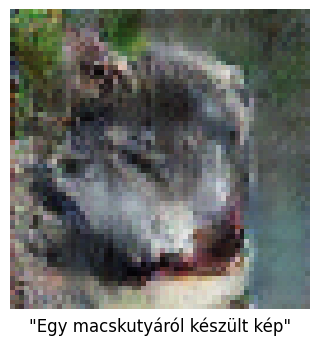
\includegraphics[width=6cm]{images/demo1.png}
	\caption{Demo kép}
	\label{fig:demo}
\end{figure}

A fejezetben be kell mutatni, hogy az elkészült alkalmazás hogyan használható.
(Az, hogy hogyan kell, hogy működjön, és hogy hogy lett elkészítve, az előző fejezetekben már megtörtént.)

Jellemzően az alábbi dolgok kerülhetnek ide.
\begin{itemize}
	\item Tesztfuttatások. Le lehet írni a futási időket, memória és tárigényt.
	\item Felhasználói kézikönyv jellegű leírás. Kifejezetten a végfelhasználó szempontjából lehet azt bemutatni, hogy mit hogy lehet majd használni.
	\item Kutatás kapcsán ide főként táblázatok, görbék és egyéb részletes összesítések kerülhetnek.
\end{itemize}